% $Id$

\chapter{Introduction}
\label{chap:intro}
\minitoc

%==========================
\section{Background}
%==========================

Advances in neuroimaging techniques have radically changed the way neuroscientists address questions about functional anatomy, especially in relation to behavioural and clinical disorders. Many questions about brain function, previously investigated using intracranial electrophysiological recordings in animals can now be addressed non-invasively in humans. Such studies have yielded important results in cognitive neuroscience and neuropsychology. Amongst the various neuroimaging modalities available, Magnetic Resonance Imaging (MRI) has become widely used due to its relatively high spatial and temporal resolution, and because it is safe and non-invasive. By selecting specific MRI sequence parameters, different MR signals can be obtained from different tissue types, giving images with high contrast among organs, between normal and abnormal tissues and/or between activated and deactivated brain areas. MRI is often sub-categorized into structural MRI (MRI) and functional MRI (fMRI). Positron Emission Tomography (PET) is another example of neuroimaging modality which measures metabolic processes. Examples of other of imaging modalities that measure  brain signals are ElectroEncephaloGraphy (EEG) recordings and MagnetoEncephaloGraphy (MEG) recordings. Neuroimaging data are inherently multivariate, since each measure (scan or recording) contains information from thousands of locations (e.g. voxels in MRI or electrodes in EEG). Considering that most brain functions are distributed processes involving a network of brain regions, it would seem desirable to use the spatially distributed information contained in the data to give a better understanding of brain functions in normal and abnormal conditions.
\\

The typical analysis pipeline in neuroimaging is strongly rooted in a mass-univariate statistical approach, which assumes that activity in one brain region occurs independently from activity in other regions. Although this has yielded great insights over the years, specially in terms of function localization, and continues to be the tool of choice for data analysis, there is a growing recognition that the spatial dependencies among signal from different brain regions should be properly modelled. The effect of interest can be subtle and spatially distributed over the brain - a case of high-dimensional, multivariate data modelling for which conventional tools may lack sensitivity. 
\\

Therefore, there has been an increasing interest in investigating this spatially distributed information using multivariate pattern recognition approaches, often referred to as  multi-voxel pattern analysis (MVPA) (see  \cite{Norman2006},  \cite{Haynes2006} and \cite{Pereira2009}). Where pattern recognition has been used in neuroimaging, it has led to fundamental advances in the understanding of how the brain represents information and has been applied to many diagnostic problems. For the latter, this approach can be used to predict the group membership of the patient scanned (healthy vs. patients or disease A vs. B) and can provide the discriminating pattern leading to this classification. Pattern recognition techniques can also be used to identify relationships between patterns of brain structure or activity and continuous measures such as age or a clinical score. Such information can then be used to predict individual-level measures for new individuals (i.e. regression models).
\\

Several active areas of research in machine learning are crucially important for the difficult problem of neuroimaging data analysis: modelling of high-dimensional multivariate time series, sparsity, regularisation, dimensionality reduction, causal modelling, and ensembling to name a few. However, the application of pattern recognition approaches to the analysis of neuroimaging data is limited mainly by the lack of user-friendly and comprehensive tools available to the fundamental, cognitive, and clinical neuroscience communities. Furthermore, it is not uncommon for these methods to be used incorrectly, with the most typical case being improper separation of training and testing datasets.
\\

\noindent \textbf{Note:} PRoNTo (Pattern Recognition for Neuroimaging Toolbox) is first and foremost a machine learning tool used for neuroimaging analyses, so throughout the manual we mostly refer to examples that focus on neuroimaging data. That being said, since from the current release PRoNTo supports MEEG (SPM) data as well as any .mat file, one can use PRoNTo to analyze for example MEEG data in sensor space (2D, or even 1D), or yet any kind of .mat file, such as behavior data. However, it is best to use PRoNTo primarily for neuroimaging data which is its original purpose or to build multi-modal predictive models including imaging and non-imaging information. So from the current release, we will refer to our data with the general term `samples' and `features', instead of referring to `voxels' as our features. The reason is that from the current release we have expanded our functionalities to include data that are not 3D, and therefore they do not have `voxels' as features.
\\

%==========================
\section{Methods}
%==========================

PRoNTo (Pattern Recognition for Neuroimaging Toolbox) is a toolbox based on pattern recognition techniques for the analysis of neuroimaging data. Statistical pattern recognition is a field within the area of machine learning which is concerned with automatic discovery of regularities in data through the use of computer algorithms, and with the use of these regularities to take actions such as classifying the data into different categories \cite{Bishop2006}. In PRoNTo, brain images are treated as spatial patterns and statistical learning models are used to identify statistical properties of the data that can be used to discriminate between experimental conditions or groups of subjects (classification models) or to predict a continuous measure (regression models).
\\

PRoNTo is \matlab-based and includes six main modules: `Data \& Design', `Prepare feature set', `Model: Specify new', `Model: Specify from', `Model: Run' and `Compute weights'. For a specific model PRoNTo can display results in terms of performance as well as  the model's weights. Additional review options enable the user to review information about the data, features and models. All modules were implemented using a graphical user interface (GUI) and the \matlab{}  Batch System. Using the \matlab{}  Batch System the user can run each module as batch jobs, which enables a very efficient analysis framework.  All information about the data, experimental design, models and results are saved in a structure called PRT. PRoNTo also creates additional files during the analysis that are described in details in the next chapters.
\\

The toolbox code is distributed for free, but as copyright software under the terms of the GNU General Public License as published by the Free Software Foundation. 

\subsection{Inputs and preprocessing}

In terms of neuroimaging modalities, PRoNTo accepts NIfTI files, which are files mostly designed to analyse structural and functional MRI as well as PET. In case of NIfTI files, it assumes that the neuroimaging data has been previously pre-processed using SPM (\url{http://www.fil.ion.ucl.ac.uk/spm/}) or a similar software for neuroimaging analysis. In general, raw fMRI data should be previously corrected for movement artefact (realigned) and time difference in slice acquisition (slice time correction), mapped to a common template (normalized) and spatially smoothed. The normalisation and spatial smoothing steps might not be necessary for single subject analysis. In addition, the General Linear Model (GLM) can be applied as a pre-processing step for pattern recognition analysis. In this case, the GLM coefficients (e.g. beta or contrast images from SPM) will correspond to the spatial patterns. Using beta images should be preferred instead of raw data in the case of event-related designs with short inter-stimulus time and/or event duration to better take into account the Haemodynamic Response Function (HRF). \textbf{Important note}: Beta images output by SPM contain NaNs (Not a Number) values in some voxels/features. For better performance of the model, a mask should be created to exclude the corresponding voxels/features from the analysis. Practically, a mask should be built (e.g. using SPM imcalc batch or a script provided in `utils') to specify which voxels/features have scalar values (0 and 1 in mask) or NaN. The updated mask should then be input in the Data \& Design window. To ease this extra preprocessing step, a script is provided in the PRoNTo folder \textit{utils}. It takes as inputs the images (i.e. beta images in NIfTI format), the mask to update (e.g. SPMnoeyes.nii provided in the PRoNTo folder \textit{mask}) and the directory to save the updated mask. Inputs are optional, and just typing in the \matlab{} command: prt\_utils\_update\_mask will ask for the different inputs using file and path selectors.
\\

% In the current version of the software, regression models and regressing out effect of covariates from the data is provided only when selecting images by scans (i.e. for one image per subject). Therefore, we suggest that users interested in removing covariates from datasets with a (fMRI) design perform a GLM analysis before hand and input the derived beta images as patterns. XXXX[needs changing]
% \\

Raw structural MRI data should be previously mapped to a common template (normalized) and spatially smoothed. Raw PET data should be realigned, normalized and smoothed. PET data is also usually scaled. This operation can be performed before hand or during the building of the feature set.
\\

Another type of neuroscience data supported by PRoNTo is electrophysiological data. These can be 1D or 2D EEG, MEG, LFP or ECoG. PRoNTo accepts this type of data in the MEEG data format, which is the standard data format created and used by SPM. PRoNTo assumes that this data format represents a within-subject design and it will read all the information automatically. The data has to contain epoched trials, either one per stimulus or one per condition. Only one MEEG file can be entered per subject and modality.
\\

The third data format supported by PRoNTo is .mat files. For example, 1D or 2D psychometric data, or connectivity matrices, can be built in .mat files, according to PRoNTo specifications, and analyzed. The variables need to be numerical (no categorical inputs) and saved as an array or vector in the first variable of the file, with no restriction on the dimensions.
\\

A limitation PRoNTo has is that for some computational reasons it cannot accept the standard format that is usually used for data of this type, i.e. \#samples/subjects X \#features. Instead, it required one .mat file per sample/subject. PRoNTo provides scripts where one can easily do these operations. Furthermore, the dimensionality of the data needs to be consistent across samples, i.e. same number of dimensions and variables in the same order.
\\

Finally, the model weights can be displayed only for 1D and 2D MEEG or .mat inputs. The display has not been specialized for MEEG as there are many much better tools to explore such files, either directly in SPM or converting back to your favourite software.

\subsection{Machine learning algorithms}

In PRoNTo different pattern recognition algorithms correspond to different machines. The machine library in PRoNTo v3.0 includes three pattern classification algorithms: Support Vector Machine (\cite{Cristianini2000}, \cite{Mourao-Miranda2007}), Gaussian Process Classifier (binary and multiclass, \cite{Rasmussen2006}, \cite{Marquand2010}) and L1 Multi-Kernel Learning \cite{Rakotomamonjy2008}. There are also five pattern regression algorithms available: Kernel Ridge Regression \cite{ShaweTaylor2004}, Relevance Vector Regression \cite{Tipping2001}, Gaussian Process Regression \cite{Rasmussen2006}, linear epsilon-insensitive SVM ($\epsilon$-SVM) regression, and L1 Multi-Kernel regression \cite{Rakotomamonjy2008}. From the current release there is also the option of using non-kernel machines in addition to the kernel ones. So there are 5 available non-kernel classification algorithms: Binary SVM using L1 and L2 loss, Multiclass SVM, as well as Logistic Regression using L1 and L2 loss (\cite{chang2011libsvm, fan2008liblinear}). Finally, for regression there is only the linear epsilon-insensitive SVM ($\epsilon$-SVM) at the moment.
\\


PRoNTo was developed with the aim of facilitating the interaction between machine learning and the neuroimaging communities. On one hand the machine learning community should be able to contribute to the toolbox with novel published machine learning models. On the other hand, the toolbox should provide a variety of tools for the neuroscience and clinical neuroscience communities, enabling them to ask new questions that cannot be easily investigated using existing statistical analysis tools. 


%=====================
\section{Installing \& launching the toolbox}
%=====================
\label{sec:Installation}

In order to work properly, PRoNTo requires 2 other softwares:
\bi
\item A recent version of \matlab. We used versions 7.5 (R2007b) to 9.4 (R2018a) to develop PRoNTo, and PRoNTo will not work with earlier versions\footnote{Any later \matlab{}~version should work, {\it in principle}.}. The statistics toolbox of \matlab{} is also required. Note: Windows and Mac users may encounter compiler issues when using R2016b and R2017b. Files may need to be compiled again. Users can install the \matlab{} required compiler from Add-Ons, or by manually downloading \href{https://www.mingw-w64.org/}{MinGW}.

\item SPM12 \cite{SPM8} installed on your computer\footnote{SPM12 can be dowloaded from the following website: \url{http://www.fil.ion.ucl.ac.uk/spm/software/}.  You should install it in a suitable directory, for example {\tt C:\bslash SPM12\bslash }, then make sure that this directory is on the \matlab{} path. No need to include the subdirectories!}. Users are recommended to have the latest updates by typing: spm\_update (check if there are new updates available) and spm\_update update (start updating files). \textbf{Important note}: if you already have a version of SPM on your computer, please update it. Various bugs, especially in terms of weight visualization, arise from out of date SPM versions.
\ei

PRoNTo latest public version can be downloaded, after registration, from the following address: \url{http://www.mlnl.cs.ucl.ac.uk/pronto/prtsoftware.html}.


\subsection{Installation}
%--------------------------------------

After downloading the zipped file containing PRoNTo, the installation proceeds as follow:
\begin{enumerate}\addtolength{\itemsep}{-1\baselineskip}
\item	Uncompress the zipped file in your favourite directory, for example {\tt C:\bslash PRoNTo\bslash };\\
\item	Launch \matlab;\\
\item	Go to the ``{\tt File}'' menu $\rightarrow$ ``{\tt Set path}'';\\
\item	Click on the ``{\tt Add folder}'' button and select the PRoNTo folder, i.e. {\tt C:\bslash PRoNTo\bslash } if you followed the example;\\
\item	Click on save.
\end{enumerate}

Some routines, in particular the `machines', are written in C++ ({\tt .cpp} files) for increased efficiency. We are trying to provide these compiled routines for the usual Operating Systems (OS's) such as: Windows XP (32 bits), Windows 7/10 (64 bits), Mac OS 10 and Linux (32 and 64 bits). If your OS is not listed or routines do not work properly then you should compile the routines for your specific OS. 

\subsection{Launching and batching}
%--------------------------------------

Once installed, there are three ways to call up PRoNTo functionalities.
To launch the toolbox GUI, just type {\tt prt} or {\tt pronto} at the \matlab{} \ prompt and the main GUI figure will pop up, see Fig.~\ref{fig:mainGUI}. From there on simply click on the processing step needed (see Part \ref{sec:part_1} of this manual). Most functions of PRoNTo have been integrated into the {\tt matlabbatch} batching system \cite{matlabbatch} (like SPM8) and the batching GUI is launched from the main GUI by clicking on the {\tt Batch} button  (see Part \ref{sec:BATCH} of this manual).
Of course most tools can also be called individually by calling them directly from the \matlab{} \ prompt, or for scripting in a {\tt .m} file  (see Part \ref{sec:ADVTOP} of this manual).

\begin{figure}[!htbp]
  \begin{center}
      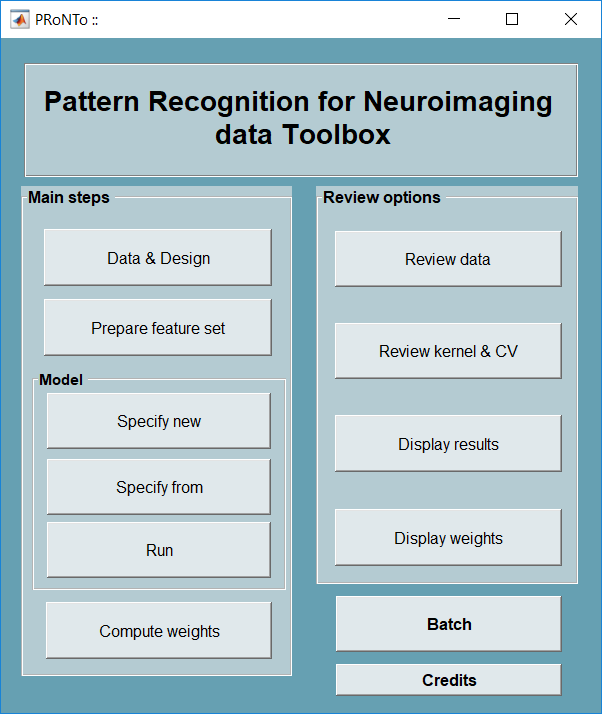
\includegraphics[height=7cm]{images/Tutorial/v3/main_prt.png}
   \caption{Main GUI interface: each button launches a specific processing step.}
    \label{fig:mainGUI}
  \end{center}
\end{figure}

\subsection{Troubleshooting}
%--------------------------------------

MEX files are provided for 64 bit Windows, MacOS and Linux (Ubuntu/Debian) systems. However, if your system specifications do not align with those above, making new MEX files is necessary. In such cases you will most likely hit an error. Please follow the instructions below in case this happens.

\subsubsection{Compiling LIBSVM}
Some problems when using SVMs might also arise due to LIBSVM, in which case, you might need to compile it on your own. The first thing that needs to be done is to download the desired LIBSVM version (usually the latest one) from the following website: \url{http://www.csie.ntu.edu.tw/~cjlin/libsvm/}. Then, the process will depend on your operating system.

If the steps described bellow do not work, please refer to the {\tt README} file that comes with LIBSVM.

\paragraph{Microsoft Windows}
\begin{itemize}
    \item Make sure you have a C++ compiler install. If not, you can install Microsoft Visual C/C++;
    \item Copy the libsvm folder to the `machines' directory of your PRoNTo instalation\\(e.g. C:\bslash PRoNTo\bslash machines\bslash);
    \item Open a DOS command window and change to the libsvm folder in the previous step ({\tt cd C:\bslash PRoNTo\bslash machines\bslash libsvm-3.17\bslash}). If the environment variables of VC++ have not been set, run the following command:\\{\tt C:\bslash Program Files\bslash Microsoft Visual Studio 10.0\bslash VC\bslash bin\bslash vcvars32.bat}. This command might be different, depending on the path of your Visual Studio installation;
    \item In the libsvm folder run the command: {\tt nmake -f Makefile.win clean all} 
    \item If no errors appear, open \matlab;
    \item Change to the `matlab' folder inside the libsvm folder (e.g. C:\bslash PRoNTo\bslash machines\bslash libsvm-3.17 \bslash matlab\bslash);
    \item Run {\tt make} in the \matlab{} Command Window. If there are no errors, you have just successfully compiled LIBSVM to be used with \matlab.
\end{itemize}

Remember, if you want to use the version that you have just compiled, you have to add the libsvm folder to your path in \matlab. If you have more than one libsvm folder inside the `machines' folder, please remove one of them from the \matlab{} path. You should only have one libsvm folder in your path.


\paragraph{Unix (Mac OS or Linux)}

\begin{itemize}
    \item Make sure you have a C++ compiler installed. If you are using Mac OS, please install `Xcode'. On Linux systems, you should already have `gcc' installed;
    \item Copy the libsvm folder to the `machines' directory of your PRoNTo instalation\\(e.g. {\tt /home/<username>/PRoNTo/machines/});
    \item Open a terminal window and change to the `machines' directory: {\tt cd PRoNTo/machines/}
    \item Compile libsvm by running the following command: {\tt make}
    \item If no errors appear, open \matlab;
    \item Change to the `matlab' folder inside the libsvm folder (e.g. PRoNTo/machines/libsvm-3.17/matlab/);
    \item Run {\tt make} in the \matlab{} Command Window. If there are no errors, you have just successfully compiled LIBSVM to be used with \matlab.
\end{itemize}

Remember, if you want to use the version that you have just compiled, you have to add the libsvm folder to your path in \matlab. If you have more than one libsvm folder inside the `machines' folder, please remove one of them from the \matlab{} path. You should only have one libsvm folder in your path.

\subsubsection{Compiling GPML}
In case there are compiler problems when using GPs due to GPML, you will need to compile it on your own. The instructions to do so are approximately the same as with LIBSVM.

\bi
\item Inside \matlab, change to the `util' folder inside the gpml folder (e.g. PRoNTo/machines/gpml/gpml-matlab-v3.5-2014-12-08/util/);

\item Run {\tt make} in the \matlab{} Command Window. If there are no errors, you have just successfully compiled GPML to be used with \matlab.
\ei


%==========================
\section{What's new?}
%==========================

\subsection{Version 3.0}
\label{ssec:whats_new_v3}

This version of the toolbox has a new layout, and includes multiple new features and functionalities. Below is a list of selected major changes and new functionalities:
\\

\noindent \underline{\textbf{File formats}}
\\

PRoNTo now accepts multiple `Data formats', i.e. NIfTI (as before), .mat and MEEG SPM data.

\begin{itemize}

\item \textbf{MEEG:} These can be 1D or 2D EEG, MEG, LFP or ECoG files converted to the MEEG SPM data format and can be entered when choosing `Select by Subject'. PRoNTo assumes that this file format represents a within-subject design that it will read automatically. The data has to contain epoched trials, either one per stimulus or one per condition. Only one MEEG file can be entered per subject and modality.

\item \textbf{.mat:} Any set of variables can be saved in a .mat and used in PRoNTo. The variables need to be numerical (no categorical inputs) and saved as an array or vector (no restriction on dimension) in the first variable of the file. One .mat needs to be provided per sample. The dimensionality of the data needs to be consistent across samples (i.e. same number of dimensions and variables in the same order). The model weights can be displayed only for 1D and 2D MEEG or .mat inputs. The display has not been fine-tuned for MEEG as there are many tools available to display such files (either directly in SPM or converting back to your favourite software).

\end{itemize}

\noindent \underline{\textbf{Combine multiple types of data}}
\\

In previous versions of PRoNTo, modalities could only be combined if they had the same number of features. The framework has been modified to allow the combination of modalities with different number of features at the model level. The option for `building one kernel per modality' in the `Prepare feature set' module has been removed. This means that, at the feature set step, only runs of a same data format can be concatenated as samples. At the model step, multiple feature sets can now be included in a model. These will be either concatenated (if a single kernel machine is selected) or used in multiple kernel settings during model estimation.
\\

\textbf{Important note:} when combining multiple feature sets, the number (and the order) of the samples need to be identical across feature sets. This means that if there are 3 conditions in the MEEG data saved as `condB', `condA', `condC', then it is not enough for the equivalent beta images for fMRI to include the conditions `condA', `condB' and `condC'. These also need to be entered in the exact same order! It might not throw an error but will lead to poor performance of the model.
\\

\noindent \underline{\textbf{Subsampling classes}}
\\

PRoNTo now allows to subsample classes to match the number of samples in the smallest class (or as close as possible) while taking into account the stratified structure of the data (e.g. blocks of scans in fMRI) as well as potential pooling of multiple conditions (i.e. it will subsample equally from all pooled conditions). Related to this option, a new module has been implemented: `Specify from'. This module (batch and GUI) allows to choose a model that has been previously specified as a `basis' for a new model. Some fields of this `basis' model will be copied into the new model, including class or regression sample selection and outer cross-validation. This ensures that, when performing subsampling, the exact same samples are considered in the `basis' model and in the new model to ease performance comparison.
\\

\textbf{Important note:} Subsampling uses the standard random number generator implementations of \matlab. Different issues have been reported about the generation of different random sequences across different Operating Systems, or even different versions of the same Operating Systems due to various reasons, which could affect your results and their reproducibility. If total reproducibility is a must, the user is advised to set their own random number generator. This can be done by modifying the script $prt\_model.m$ in line \#338 where the standard random number generator is set.
\\[0.4cm]

\noindent \underline{\textbf{Machines}}

\begin{itemize}

\item \textbf{Kernel machines:} PRoNTo interfaces LIBSVM. However, only the SVM algorithm was used so far. PRoNTo now interfaces LIBLINEAR as well and uses more algorithms from both libraries. In addition, the `custom' machine can now be optimized given hyper-parameters. PRoNTo also allows the optimization of more than one parameter (entered as a cell array of values that is then transformed into a grid).

\item \textbf{Non-kernel machines:} The non-kernel route has also been enabled, i.e. the `Use kernel' radio button can be ticked off to use primal formulations instead of kernel machines. This is intended for samples with a low number of features. Please note that using these algorithms on typical neuroimaging datasets (i.e. \# features $>>$ \# samples), will likely lead to time-consuming estimations and poor performance.

\end{itemize}

\noindent \underline{\textbf{Regression targets}}

\begin{itemize}

\item \textbf{Per subject:} Multiple regression targets can be specified at the Data \& Design level. When choosing which samples to use for the regression model, the user can also specify which target to use. This avoids the need for multiple PRT files when multiple regression targets might be of interest.

\item \textbf{Per trial:} Regression targets can be input along the conditions of an experimental design to perform within-subject regression.

\end{itemize} 

\noindent \underline{\textbf{Cross-validation}}
\\

A `Leave-One-Block-per-Class-Out' cross-validation scheme was added with its k-folds counterpart to allow balanced train and test sets when performing within subject cross-validation.
\\

\noindent \underline{\textbf{Other important changes}}
\\

\begin{itemize}
\item \textbf{Model performance estimation:} Model performance was computed based on the concatenation of predictions across folds. This way to estimate model performance can however lead to over-optimistic model performance estimations and further reflects a model that was not estimated (instead, we estimated multiple models). We have hence modified the code to compute the average of performance across folds. This is also reflected in the `Display results' window where some plots have been replaced at the model level (e.g. replacing the overall confusion matrix by a `balanced accuracy distribution' across folds in the plot). In general, the results will reflect more the average but also the deviation of the results across folds. We encourage the users to report both values.
Furthermore, there has also been a change in the way we compute the normalized MSE. Until PRoNTo v2.1, the MSE was normalized by dividing it with the range of values ($max(targets) - min(targets)$). The main disadvantage of this was that in the case of spurious outliers, the results were not representative of how good the model fit the data. So from PRoNTo v3.0 the MSE is normalized by dividing the MSE with the $variance$ of the target values.

\item \textbf{Gaussian Process Regression:} Until PRoNTo v2.1, the covariance matrix used was $k(x,z) = (x'*z)/t2$ with \textit{t2} being the optimizable hyperparameter controlling the scaling of the latent function. After some empirical results showing that this covariance matrix was overparameterized, from PRoNTo v3.0 we change the covariance matrix to $k(x,z) = (x'*z)$, which has no hyperparameters.


\item \textbf{Hyper-parameter optimization:} This change only applies when multiple values of the hyper-parameter lead to the same maximum value of model performance. In previous versions, PRoNTo was choosing the median value. In v3.0, PRoNTo identifies the largest stable region (if the `Image Processing' toolbox from \matlab{} is present) and chooses the center of gravity of this region in the hyper-parameter grid as the best hyper-parameter. This change should have limited impact on the results.

\item \textbf{Increased flexibility:} Many checks and errors have been simplified or discarded to allow more flexible analyses. It however comes with the downside that it is easier to make mistakes in the analysis. Please make sure you double-check every step and regularly load the PRT to verify the input information.

\end{itemize}

\noindent \underline{\textbf{MATLAB important changes}}
\\

We noticed a change between \matlab{} versions R2017b and R2018a in the \matlab{} \textbf{norm} function which is used by PRoNTo when normalizing samples. And hence, users should be aware that when normalizing samples, results might vary between \matlab{} versions up to R2017b and from version R2018a and onwards.


\subsection{Version 2.1}
This version of the toolbox is released mainly to provide a bug-fixed version of v2.0. One new functionality is added: removing confounds. A detailed description of this procedure can be found at \url{http://www.cs.ucl.ac.uk/fileadmin/UCL-CS/research/Research_Notes/RN_17_09_ARJMM.pdf}. 

Below is a list of selected bug fixes that might affect your use of the software or previously obtained results: 
\begin{itemize}
\item \textbf{HRF delay and overlap}: In the Data\&Design module users can define parameters to approximate the HRF shape (namely HRF delay and overlap). In earlier versions, the values could only be entered once and applied to all modalities. This has now been fixed to allow different values for different modalities, in the batch and in the GUI.   
\item \textbf{Freeze the Review Data window}: In relation to the HRF delay and overlap bug fix, the Review data is now `on wait' until closed. This means that no operation (in PRoNTo or in \matlab) can be done until the window is closed. This ensures that values input in the Data review GUI are passed to the main Data and Design window.   
\item \textbf{ROC and AUC}: There was a bug in how we computed the area under the curve (AUC) and plotted the receiver operating characteristic (ROC) curve that we have now fixed. This means that different AUC values and ROC plots might be observed, if comparing previously obtained results in older versions and in v2.1. We hence recommend re-computing AUC and re-plotting ROC if needed. 
\item \textbf{k-fold CV}: Before v2.1, when using k-fold cross validation (CV) and the number of samples was not divisible by k, we re-allocated the remainder to the last fold by default. For example, a 4 fold CV with 43 samples would lead to 4 folds of size 10,10,10 and 13 respectively. In v2.1, the remainder is evenly re-allocated to each fold, starting from the first. The above example would then lead to folds of size 11, 11, 11 and 10. This change affects all k-fold CV scheme and should then be taken into consideration if comparing results from older versions with results from v2.1.  
 
\end{itemize}

\subsection{Version 2.0}
This version of the toolbox (2015) aims at providing multiple new functionalities, including:
\begin{itemize}
\item \textbf{Build one kernel per modality}: When there are multiple modalities in the same dataset, it is now possible to build one kernel per modality and use them in the same model later on. If this option is not chosen, the selected modalities can still be concatenated as additional samples/examples or sessions (if they have the same features) or used separately.
\item \textbf{Build one kernel per region}: It is also possible to specify an atlas, comprising regions of interest (ROIs) as defined by values in the atlas ranging from 1 to \textit{number of ROIs}. For each anatomically defined ROI, a kernel will be built taking into account the multivariate pattern within the region. It is possible to use this feature in combination with the previous one (e.g. one kernel per region and per modality, or concatenate modalities as additional samples and build one kernel per region).
\item \textbf{New machines}: The list of available machines was extended, and now includes L1 Multi-Kernel Learning (MKL, classification and regression). The latter corresponds to a hierarchical model defined by weights at two levels: the feature level and the kernel level (i.e. ROI and/or modality).
\item \textbf{Flexible cross-validation}: A GUI is provided to manually specify a custom cross-validation matrix. It allows to either specify a basis (e.g. leave-one-subject-out), load a .mat or specify the number of folds. Then the user can, for each fold, select which examples are part of the training set, test set, or won't be used. The resulting matrix can be saved for further use.
\item \textbf{Nested cross-validation for hyperparameter optimization}: It is now possible to optimize the hyperparameter(s) of some machines (e.g. the soft-margin parameter, C, in SVM) using a nested cross-validation (CV) framework. The number of folds in the nested cross-validation, used only to estimate the value of the hyperparameter leading to the highest performance, does not need to be the same as the `outer' cross-validation (i.e. the one estimating the final model performance). For example, to decrease computational expenses, the nested CV can be a 4-fold CV while the outer CV can be a leave-one-out.
\item \textbf{Display results}: The display of the results was divided into two modules (Display Results and Display Weights). This allows to review the model performance in one window, with all the statistics. A new graph displaying the effect of the hyperparameter (if optimized) was also included.
\item \textbf{Weights per ROI}: For each model it is possible to build images representing the weights per feature and also images summarising the weights per regions of interest as defined by an atlas. If an MKL model was built on ROIs, the contribution of each ROI (regional weight) is explicitly derived. On the other hand, if a simple kernel model was selected (e.g. SVM on the whole brain), the weights per feature will be averaged (in absolute value) within each region, as defined by an atlas specified by the user. In both cases, an additional image, with weights per ROI, is created and saved.
\item \textbf{Display weights}: The weights of each model can be displayed at the feature level in this window. If weights per ROI were derived (either summarized or from an MKL on ROIs), weights per region can be displayed as an image, as well as in a sorted list of regions. The same applies for MKL models on multiple modalities. A histogram is also displayed representing the contribution/weight of each ROI/modality to the model. The table can be exported as text for future use in publications/communications.
\end{itemize}

\subsection{Version 1.1}
In 2012, PRoNTo v1.1 was released mainly to provide bug fixes for version v1.0. Two features were also added:
\begin{itemize}
\item automatic compiling of the machines (in particular: no more issues with SVM, nor with \matlab{} toolboxes and paths).
\item k-folds Cross-Validation (CV): specify the number of folds or set it to 1 for half-half CV (train on first half, test on second).
\end{itemize}

\subsection{Version 1.0}
Launched in 2011, this version of PRoNTo allows to perform all the analysis steps, from Data \& Design to computing the weights for three classification machines (SVM, binary and multi-class GP) and two regression machines (KRR, SVR).

%==========================
\section{How to cite}
%==========================
Please cite: 

\bi
\item Schrouff J, Rosa MJ, Rondina JM, Marquand AF, Chu C, Ashburner J, Phillips C, Richiardi J, Mourao-Miranda J. \href{https://doi.org/10.1007/s12021-013-9178-1}{PRoNTo: Pattern Recognition for Neuroimaging Toolbox}. Neuroinformatics, 2013, 11(3), 319-337.
\ei

\bi
\item Schrouff J, Mourao-Miranda J, Phillips C, \& Parvizi J. \href{https://doi.org/10.1016/j.jneumeth.2015.11.028}{Decoding intracranial EEG data with multiple kernel learning method}. Journal of neuroscience methods, 2016, 261, 19-28. 
\ei

\noindent When using PRoNTo analyses in any type of publication. In addition, when using Multiple Kernel Learning to combine signals from different Regions of Interest (ROIs) or modalities, one should also refer to the following publication: 

\bi
\item Schrouff J, Monteiro, JM, Portugal L, Rosa MJ, Phillips C, Mourao-Miranda J. \href{https://doi.org/10.1007/s12021-017-9347-8}{Embedding Anatomical or Functional Knowledge in Whole-Brain Multiple Kernel Learning Models}. Neuroinformatics, 2018, 16(1), 117-143. 
\ei

\noindent And finally when using a posteriori weight summarization with atlas-defined regions of interest one should also refer to:

\bi
\item Schrouff J, Cremers J, Garraux G, Baldassarre L, Mourao-Miranda J, Phillips C. \href{https://doi.org/10.1109/PRNI.2013.40}{Localizing and Comparing Weight Maps Generated from Linear Kernel Machine Learning Models}. International Workshop on Pattern Recognition in Neuroimaging (PRNI), 2013, 124-127, DOI: 10.1109/PRNI.2013.40.
\ei



%==========================
\section{PRoNTo History}
%==========================

The first version of the `Pattern Recognition for Neuroimaging Toolbox', aka. PRoNTo, was developed in 2011 by an international team of researchers (the PRoNTo development group) led by Prof Janaina Mourao-Miranda and supported by the European Union through the PASCAL Harvest programme (\href{https://cordis.europa.eu/project/id/216886}{PASCAL2}).
\\

The original development group included Janaina Mourao-Miranda, Christophe Phillips, Jessica Schrouff, John Ashburner, Maria Joao Rosa, Jonas Richiardi, Andre Marquand, Jane Rondina and Carlton Chu. The motivation to develop PRoNTo stemmed from the unmet need of a flexible pattern recognition analysis framework that would accommodate different types of neuroimaging data, could address various research questions, and be safely used by neuroimagers who are non-expert in machine learning. As the team included \href{https://www.fil.ion.ucl.ac.uk/spm/}{SPM} developers (John Ashburner and Christophe Phillips) PRoNTo took advantage of many of the SPM existing functions, such as those for file handling and image display, as well as the batch system (\href{https://sourceforge.net/projects/matlabbatch/}{Glauch V.}).
\\

Over the years, new contributors have joined the development group and PRoNTo was further extended to include new functionalities, such as flexible cross-validation frameworks, option to remove effect of confounds, and atlas based multiple kernel learning (PRoNTo versions 1.1, 2.0, 2.1). In particular, Jessica Schrouff has been a major contributor of PRoNTo from its inception till version 3.0. PRoNTo's latest version (PRoNTo v3.0) now accepts multiple data formats and enables the building of multimodal predictive models. The latest versions of PRoNTo have been supported by the \href{http://www.wellcome.org/}{Wellcome Trust}. 
\\

Currently, the PRoNTo project is led by Prof Janaina Mourao-Miranda and co-supervised by Prof Christophe Phillips. Konstantinos Tsirlis supports the PRoNTo developments and is in charge of its management and maintenance. Contributions (e.g. new features, debugging, manual, demonstration data) are mostly provided by Prof Janaina Mourao-Miranda's group and collaborators but external contributions are welcome.


%==========================
\section{Main contributors}
%==========================
PRoNTo is  developed by the Machine Learning \& Neuroimaging Laboratory, Computer Science department, University College London, UK (\url{http://www.mlnl.cs.ucl.ac.uk}) and associated researchers.

The main contributors, in alphabetical order, are: 
\begin{description}
	\item[Dr. John Ashburner] is a Professor of Imaging Science at the Wellcome Trust Centre for Neuroimaging at the University College London Institute of Neurology. He is mainly interested in modelling brain anatomy from MR scans, and more recently in applying pattern recognition methods to make predictions about individual subjects. He is a co-developer of the SPM software (intra- and inter-subject registration, tissue classification, visualization and image file formats), which is used internationally by thousands of neuroimaging researchers. He has a Web of Science h-index of 98.  He did not contribute any actual code to PRoNTo, but he did attend many of the meetings;
    \item[Dr. Carlton Chu] is a research scientist at  Google DeepMind. Before joining DeepMind, he was a research fellow in brain imaging at the National Institute of Mental Health (NIMH), NIH. He received the B.Eng. degree (1\textsuperscript{st} class Honours) from Auckland University, in 2002 and the master of Biomedical Engineering from University of New South Wales, in 2004. Carlton obtained a PhD in Neuroimaging method from University College London in 2009, working in the statistical methods group at the Wellcome Trust Centre for Neuroimaging, creators of the famous ``SPM'' program. There he developed innovative pattern recognition methods to automatically detect the early stages of neurodegenerative diseases such as Alzheimer's and Huntingdon's from structural brain images. In 2007, Carlton won the first prize in the 2nd Pittsburgh Brain Activity Interpretation Competition (PBAIC), a prestigious international competition involving the application of machine learning to the problem of classification of brain activity. He led a small research team to victory, acclaim from peers in the field, and the \$10K first prize. His current research interests include image segmentation using convolutional neural networks and applications of deep-learning. Carlton was involved in the development of PRoNTo v1.0;
	\item[Dr. Andre Marquand] is a Principal Investigator and an assistant professor at the Donders Institute for Brain Cognition and Behaviour. His research focuses on the application of probabilistic machine learning techniques to neuroimaging data, particularly for clinical applications. His recent work includes the development of multi-class, multi-task and multi-modality pattern classification methods that offer many advantages over current techniques including more sensitive and specific detection of disease effects. He did his PhD in Clinical Neuroscience, King's College London, UK. Andre was involved in the developement of PRoNTo v1.0;
	\item[Prof Janaina Mourao-Miranda] is a Wellcome Trust Senior Research Fellow and a Professorial Research Associate at the Centre for Medical Image Computing (CMIC), Computer Science Department, UCL. Over the past years her research has involved developing and applying pattern recognition methods to analyze neuroimaging data, in particular brain activation and structural patterns that distinguish between controls and patients. Her current research focuses on developing machine-learning models to investigate complex relationships between neuroimaging data and multidimensional descriptions of mental health disorders. Janaina has been leading the PRoNTo project since 2011 and has contributed to PRoNTo v1.0, v1.1, v2.0, v2.1 and v3.0;
	\item[Dr. Joao M. Monteiro] is a former MPhil/PhD Student at University College London under the supervision of Prof John Shawe-Taylor and Dr. Janaina Mourao-Miranda. His research focused on the application of unsupervised machine learning methods to neuroimaging. He contributed to PRoNTo v1.1, v2.0 and v2.1;
	\item[Dr. Christophe Phillips] is Research Director at the GIGA Cyclotron Research Centre in vivo imaging and Associate Professor at the Department of Electrical Engineering and Computer Science, University of Li\`ege, Belgium. His research focuses on the processing of multi-modal neuroimaging data. Recent work within the field of ``brain decoding'' aimed at distinguishing between levels of consciousness in unresponsive patients or between typical and atypical Parkinson Disease patients using Positron Emission Tomography (PET) imaging, as well as tracking mnesic traces in trained healthy subjects with fMRI. Christophe contributed to PRoNTo v1.0, v1.1, v2.0, v2.1 and v3.0;
	\item[Dr. Anil Rao] was a post-doctoral researcher in Centre for Medical Image Computing (CMIC) and Max Planck University College London Centre for Computational Psychiatry and Ageing Research at the University College London. He contributed to version 2.1, in particular to the removing confounds functionality.    
	\item[Dr. Jonas Richiardi] is currently Clinical Research Lead in the Department of Radiology, Lausanne University Hospital, with a joint affiliation to Siemens Healthcare Switzerland's Advanced Clinical Imaging Technology group. He was previously a Marie Curie Fellow with a project on `Modelling and Inference on brain Networks for Diagnosis', jointly affiliated to the FINDlab at Stanford University and LabNIC at the University of Geneva. His research interests include the combination of imaging modalities with other biological information sources including genomic data, learning with graphs, machine learning for neuroimaging, brain connectivity / resting-state data analysis, interpretability of brain decoding results, and functional biomarkers. Jonas contributed to PRoNTo v1.0 and v1.1;
	\item[Dr. Jane Rondina] is a research fellow at the University College London Institute of Neurology. Previously, she was a post-doctoral research associate at the Centre for Neuroimaging Sciences, King's College London. In the past years, her research has involved application of pattern recognition methods to neuroimaging data and development of a stability-based method for feature selection and mapping in neuroimaging. Her current research focuses on prognosis and prediction of treatment response, mainly addressing approaches to combine complementary information from different imaging modalities and other sources of data (clinical, demographic and genetic). She contributed to the development of PRoNTo v1.0 and v2.0;
	\item[Dr. Maria J. Rosa] is an Advanced Support Engineer at MathWorks. Before joining Mathworks, she was an imaging scientist at IXICO, plc. Before, she was a Post-Doctoral Research Fellow at the Institute of Psychiatry, King's College London (KCL) and a Wellcome Trust post doctoral research associate at the Centre for Computational Statistics and Machine Learning (CSML), UCL. Maria's main area of work is the development and application of machine learning and multivariate methods to neuroimaging data. She did her PhD at the Wellcome Trust Centre for Neuroimaging, UCL. She contributed to PRoNTo v1.0, v1.1, v2.0 and materials for v3.0;
	\item[Dr. Jessica Schrouff] got her PhD from the University of Li\`ege, under the supervision of Dr. C. Phillips. She was a post-doctoral researcher at the Laboratory of Behavioral and Cognitive Neuroscience, Stanford University before obtaining a Marie Curie fellowship with University College London. Her research applied machine learning techniques to neuroimaging data (both cognitive and clinical neuroscience) and investigated the limitations of such models, especially in terms of interpretation. Jessica now pursues related work at Google Health. She contributed to PRoNTo versions 1.0, 1.1, 2.0, 2.1 and was a major contributor to v3.0;
	\item[Konstantinos Tsirlis] has a background in Physics, Neuroscience and Machine Learning. His M.Sc. Thesis was in Causal Structure Learning where he implemented a novel hybrid method for learning the causal structure of continuous data in the presence of latent confounders. Before joining CMIC he was involved in various computational and experimental neuroscience projects, and two causal discovery and bioinformatics projects. He is currently a Research Software Engineer in the lab, focusing on developments in PRoNTo v3.0, as well as some machine learning projects.
	\item[Dr. Tong Wu] got her PhD from the University of Queensland in Australia, under supervision of Dr. Tianzi Jiang, Dr. David Reutens and Dr. Simone Bosshard. She was a post-doctoral researcher in Centre for Medical Image Computing (CMIC) at University College London. Her research focus during PhD was resting-state mouse fMRI in both wild type mice and a schizophrenia mouse model. She contributed to PRoNTo v2.1 and was involved in PRoNTo v3.0.
	
\end{description}

We also want to thank the Laboratory of Behavioral and Cognitive Neuroscience at Stanford University for their early adoption of v3.0 and their feedback, as well as the students and post-docs for their help in testing the software and writing this manual: Fabio Ferreira, Dr Agoston Mihalik, Rafael Ramos, Dr. Juan E. Arco, Dr. Liana Lima Portugal, Liane Canas, Dr. Ana Regia Neves, Rochelle Silva, Dr. Orlando Fernandes Junior, Dr. Qinquan Gao. Finally, we would like to thank Prof Leticia de Oliveira from the Fluminense Federal University in Brazil for her suggestions to the manual and helping us extensively test PRoNTo v3.0.


%==========================
\section{Acknowledgements}
%==========================
PRoNTo is the deliverable of a Pascal Harvest project coordinated by Dr. J. Mourao-Miranda and its development was possible with the financial and logistic support of 
\begin{itemize}
\item \href{https://cordis.europa.eu/project/id/216886}{PASCAL2} and its HARVEST programme.
\item The \href{http://www.cs.ucl.ac.uk}{Department of Computer Science}, University College London.
\item The \href{http://www.wellcome.org/}{Wellcome Trust} under grants no. WT086565/Z/08/Z and no. WT102845/Z/13/Z.
\item The Fonds de la Recherche Scientifique (\href{http://www.fnrs.be}{FNRS}), Belgium.
\item Funda\c{c}\~{a}o para a Ci\^{e}ncia e Tecnologia (\href{http://www.fct.pt}{FCT}), Portugal.
\item Swiss National Science Foundation (PP00P2-123438) and Center for   Biomedical Imaging (\href{https://cibm.ch/}{CIBM}) of the EPFL and Universities and Hospitals of Lausanne and Geneva.
\item The EU Marie Curie Action under grant FP7-PEOPLE-2011-IOF \#299500 to Jonas Richiardi.
\item The EU Marie Curie Action under grant Horizon2020-2015-GF \#654038 to Jessica Schrouff.
\item The Laboratory of Behavioral and Cognitive Neuroscience (\href{https://med.stanford.edu/parvizi-lab.html}{LBCN}), Stanford University.
% \item Marie Sklodowska-Curie global fellowship to J. Schrouff (project DecoMP-ECoG, \#654038).
\end{itemize}

